\documentclass[11pt]{article}
%\usepackage{graphicx}
\usepackage{booktabs}
\usepackage[backend=bibtex]{biblatex}
%\addbibresource{myBibRefsFile.bib}
%\usepackage[backend=bibtex,style=verbose-trad2]{biblatex}
\bibliography{IT.bib}
\usepackage{float}

%\usepackage[margin=1in]{geometry}
\usepackage{fancyhdr}
%\pagestyle{fancy}
\usepackage{amsmath}
%\usepackage{amssymb}
%\usepackage[table]{xcolor}
\usepackage{bm}
\usepackage{array}
\usepackage{mathtools}
\usepackage{soul,soulutf8}
\usepackage{url,color}
\usepackage{fullpage}
\usepackage[english]{babel}

\usepackage[utf8]{inputenc}
\lhead{STA 4001: Stochastic Processes}
\chead{}
\rhead{\textup{CUHK(SZ) Fall 2018}}


\usepackage{amsmath,amsthm,amssymb}
%\usepackage{extarrows}
%\usepackage{breqn}
\usepackage{mathtools}
\DeclarePairedDelimiter\ceil{\lceil}{\rceil}
\DeclarePairedDelimiter\floor{\lfloor}{\rfloor}
\newcommand{\N}{\mathbb{N}}
\newcommand{\Z}{\mathbb{Z}}
\newcommand{\trans}{^{\mathrm T}}

\newenvironment{theorem}[2][Theorem]{\begin{trivlist}
\item[\hskip \labelsep {\bfseries #1}\hskip \labelsep {\bfseries #2.}]}{\end{trivlist}}
\newenvironment{lemma}[2][Lemma]{\begin{trivlist}
\item[\hskip \labelsep {\bfseries #1}\hskip \labelsep {\bfseries #2.}]}{\end{trivlist}}
\newenvironment{exercise}[2][Exercise]{\begin{trivlist}
\item[\hskip \labelsep {\bfseries #1}\hskip \labelsep {\bfseries #2.}]}{\end{trivlist}}
\newenvironment{reflection}[2][Reflection]{\begin{trivlist}
\item[\hskip \labelsep {\bfseries #1}\hskip \labelsep {\bfseries #2.}]}{\end{trivlist}}
\newenvironment{proposition}[2][Proposition]{\begin{trivlist}
\item[\hskip \labelsep {\bfseries #1}\hskip \labelsep {\bfseries #2.}]}{\end{trivlist}}
\newenvironment{corollary}[2][Corollary]{\begin{trivlist}
\item[\hskip \labelsep {\bfseries #1}\hskip \labelsep {\bfseries #2.}]}{\end{trivlist}}
\DeclareMathOperator{\tr}{tr}
\DeclareMathOperator{\rank}{rank}
\DeclareMathOperator{\Span}{span}
\DeclareMathOperator{\row}{row}
\DeclareMathOperator{\col}{col}
\DeclareMathOperator{\range}{range}
\DeclareMathOperator{\Null}{Null}
\DeclarePairedDelimiterX{\inp}[2]{\langle}{\rangle}{#1, #2}
\DeclareMathOperator{\Proj}{Proj}
\newcommand{\diff}{\,\mathrm{d}}
\DeclareMathOperator{\trace}{trace}
\newcommand{\Her}{^{\mathrm H}}
\DeclareMathOperator{\diag}{diag}
\newcommand{\Var}{\mathrm{Var}}
%\usepackage{listings}
%\usepackage{color} %red, green, blue, yellow, cyan, magenta, black, white
%\definecolor{mygreen}{RGB}{28,172,0} % color values Red, Green, Blue
%\definecolor{mylilas}{RGB}{170,55,241}
%
%
%\lstset{language=Matlab,%
%    %basicstyle=\color{red},
%    breaklines=true,%
%    morekeywords={matlab2tikz},
%    keywordstyle=\color{blue},%
%    morekeywords=[2]{1}, keywordstyle=[2]{\color{black}},
%    identifierstyle=\color{black},%
%    stringstyle=\color{mylilas},
%    commentstyle=\color{mygreen},%
%    showstringspaces=false,%without this there will be a symbol in the places where there is a space
%    numbers=left,%
%    numberstyle={\tiny \color{black}},% size of the numbers
%    numbersep=9pt, % this defines how far the numbers are from the text
%    emph=[1]{for,end,break},emphstyle=[1]\color{red}, %some words to emphasise
%    %emph=[2]{word1,word2}, emphstyle=[2]{style},    
%}
\usepackage{listings}
\RequirePackage{listings}
\RequirePackage{xcolor}
\definecolor{dkgreen}{rgb}{0,0.6,0}
\definecolor{gray}{rgb}{0.5,0.5,0.5}
\definecolor{mauve}{rgb}{0.58,0,0.82}
\lstset{
  frame=tb,
  aboveskip=3mm,
  belowskip=3mm,
  showstringspaces=false,
  columns=flexible,
  framerule=1pt,
  rulecolor=\color{gray!35},
  backgroundcolor=\color{gray!5},
  basicstyle={\small\ttfamily},
  numbers=none,
  numberstyle=\tiny\color{gray},
  keywordstyle=\color{blue},
  commentstyle=\color{dkgreen},
  stringstyle=\color{mauve},
  breaklines=true,
  breakatwhitespace=true,
  tabsize=3,
}

\newcommand{\degree}{\ensuremath{^\circ}}
\begin{document}
\title{\bfseries\upshape{Appendix}}%replace X with the appropriate number
\author{\textit{I will appreciate it if you could give me some advice on my final project}} %if necessary, replace with your course title
\maketitle
\section{Output Figures and Screen Printout for $s=0.1,n=3600$.}
\subsection{Output Figures ($s=0.1,n=3600$).}
\begin{figure}[H]
\centering
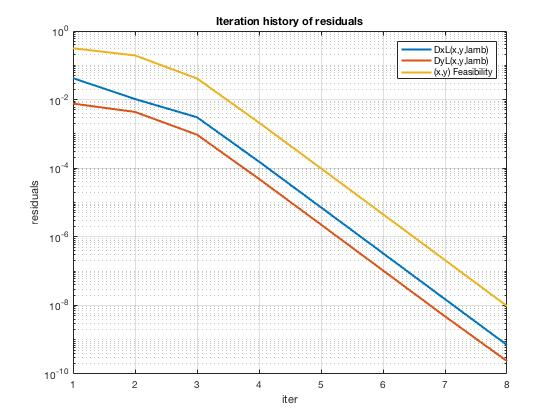
\includegraphics[width=12cm]{F_1/F_1_2.jpg}
\caption{Iteration history residuals for my code}
\end{figure}
\begin{figure}[H]
\centering
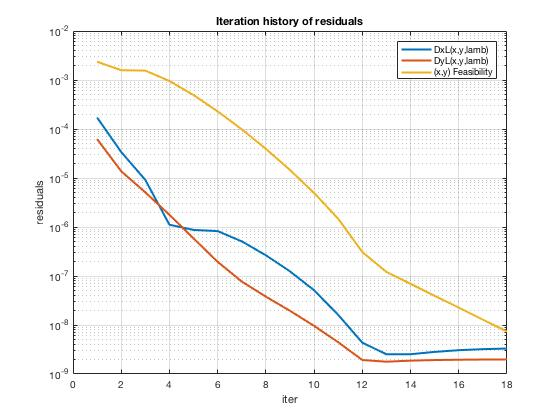
\includegraphics[width=12cm]{F_1/F_1_3.jpg}
\caption{Iteration history residuals for instructor's code}
\end{figure}

\begin{figure}[H]
\centering
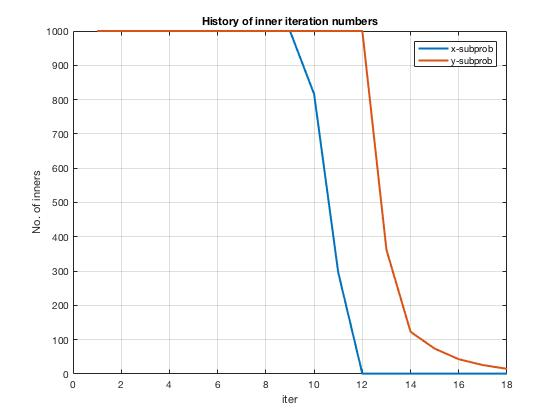
\includegraphics[width=12cm]{F_1/F_1_4.jpg}
\caption{Historty Inner iteration Numbers for instructor's code}
\end{figure}
\subsection{Screen Printout ($s=0.1,n=3600$).}
\begin{figure}[H]
\centering
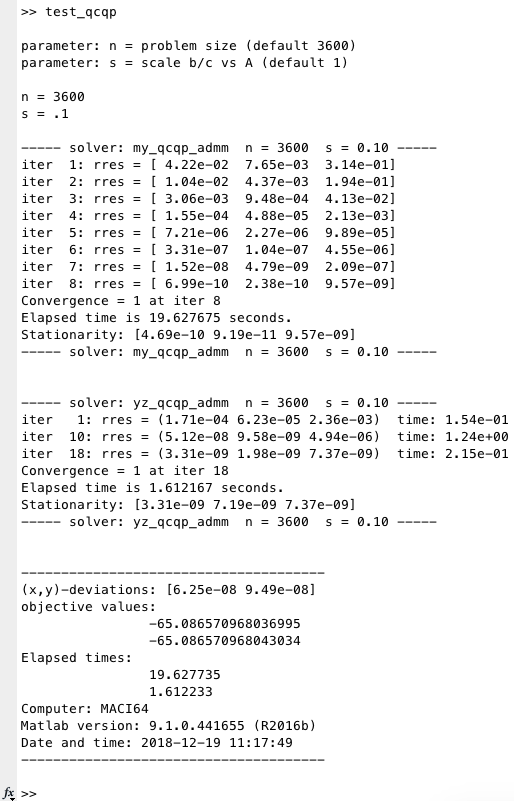
\includegraphics[width=10cm]{F_1/F_1_1.png}
\caption{Historty Inner iteration Numbers for instructor's code}
\end{figure}


\clearpage
\section{Output Figures and Screen Printout for $s=1,n=3600$.}
\subsection{Output Figures ($s=1,n=3600$).}
\begin{figure}[H]
\centering
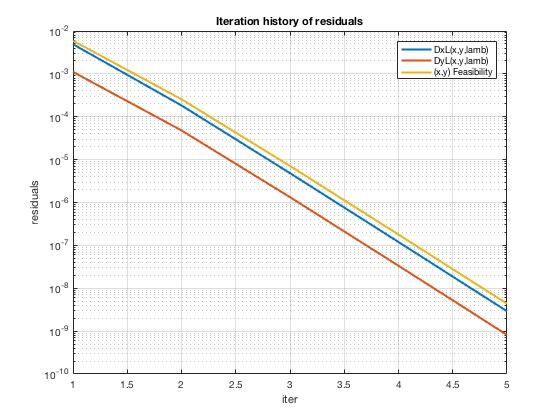
\includegraphics[width=12cm]{F_2/F_1_2.jpg}
\caption{Iteration history residuals for my code}
\end{figure}
\begin{figure}[H]
\centering
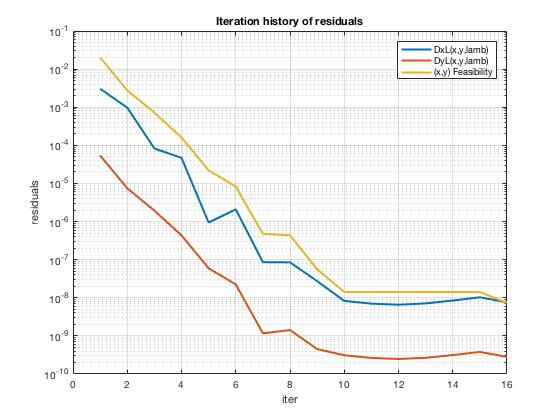
\includegraphics[width=12cm]{F_2/F_1_3.jpg}
\caption{Iteration history residuals for instructor's code}
\end{figure}

\begin{figure}[H]
\centering
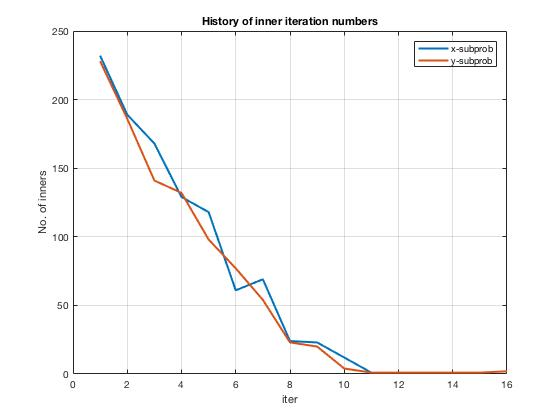
\includegraphics[width=12cm]{F_2/F_1_4.jpg}
\caption{Historty Inner iteration Numbers for instructor's code}
\end{figure}
\subsection{Screen Printout ($s=1,n=3600$).}
\begin{figure}[H]
\centering
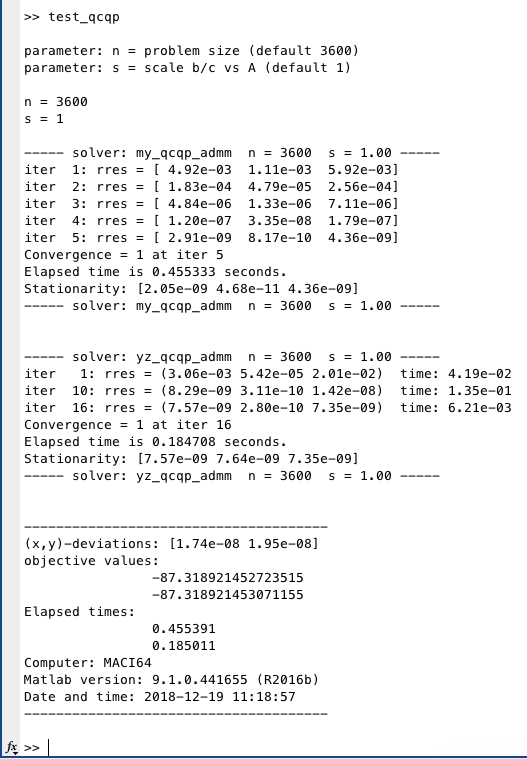
\includegraphics[width=10cm]{F_2/F_1_1.png}
\caption{Historty Inner iteration Numbers for instructor's code}
\end{figure}




\clearpage
\section{Output Figures and Screen Printout for $s=10,n=3600$.}
\subsection{Output Figures ($s=10,n=3600$).}
\begin{figure}[H]
\centering
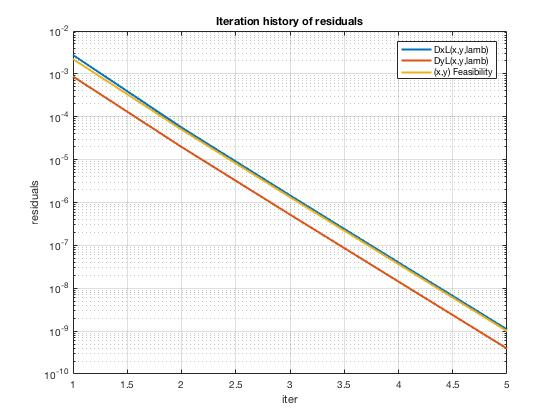
\includegraphics[width=12cm]{F_3/F_1_2.jpg}
\caption{Iteration history residuals for my code}
\end{figure}
\begin{figure}[H]
\centering
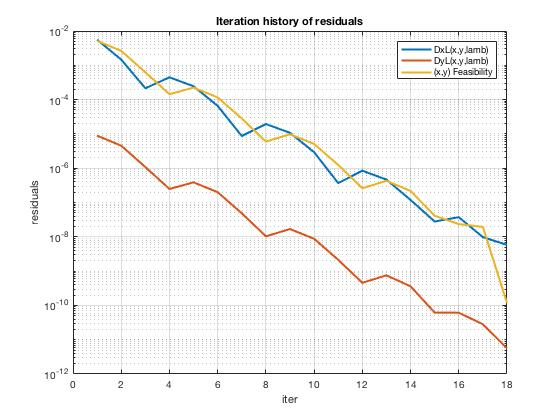
\includegraphics[width=12cm]{F_3/F_1_3.jpg}
\caption{Iteration history residuals for instructor's code}
\end{figure}

\begin{figure}[H]
\centering
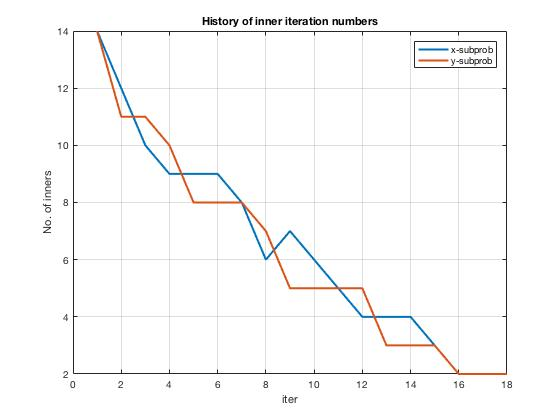
\includegraphics[width=12cm]{F_3/F_1_4.jpg}
\caption{Historty Inner iteration Numbers for instructor's code}
\end{figure}
\subsection{Screen Printout ($s=10,n=3600$).}
\begin{figure}[H]
\centering
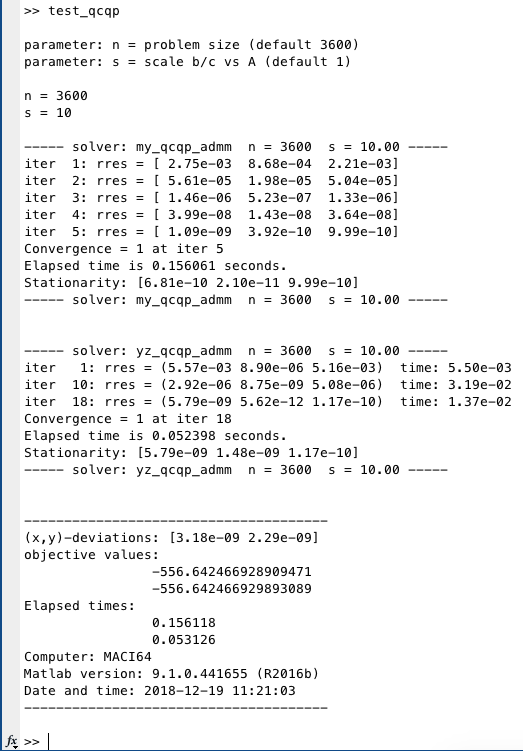
\includegraphics[width=10cm]{F_3/F_1_1.png}
\caption{Historty Inner iteration Numbers for instructor's code}
\end{figure}

\clearpage
\section{Output Figures and Screen Printout for $s=0.1,n=10000$.}
\subsection{Output Figures ($s=0.1,n=10000$).}
\begin{figure}[H]
\centering
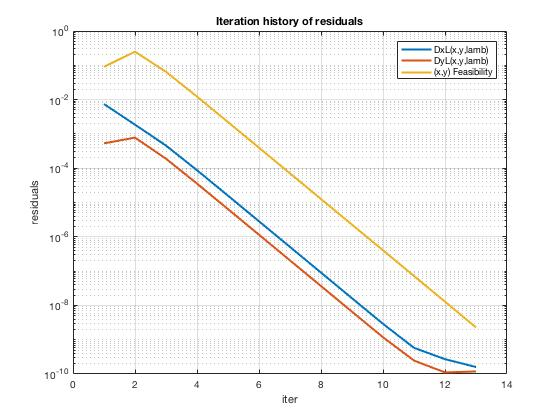
\includegraphics[width=12cm]{F_4/F_1_2.jpg}
\caption{Iteration history residuals for my code}
\end{figure}
\begin{figure}[H]
\centering
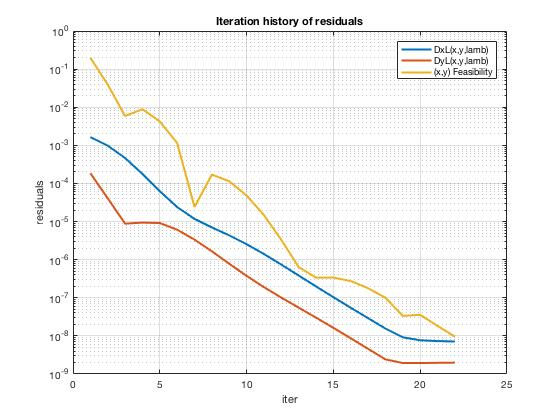
\includegraphics[width=12cm]{F_4/F_1_3.jpg}
\caption{Iteration history residuals for instructor's code}
\end{figure}

\begin{figure}[H]
\centering
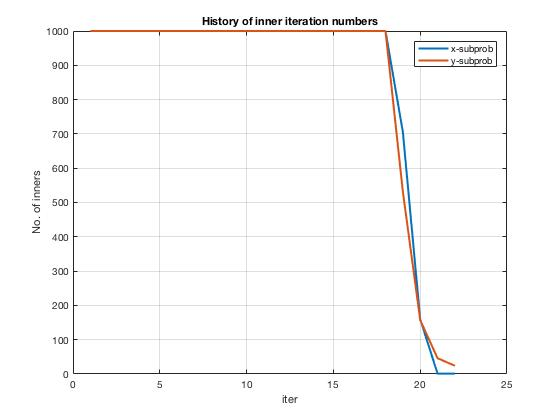
\includegraphics[width=12cm]{F_4/F_1_4.jpg}
\caption{Historty Inner iteration Numbers for instructor's code}
\end{figure}
\subsection{Screen Printout ($s=0.1,n=10000$).}
\begin{figure}[H]
\centering
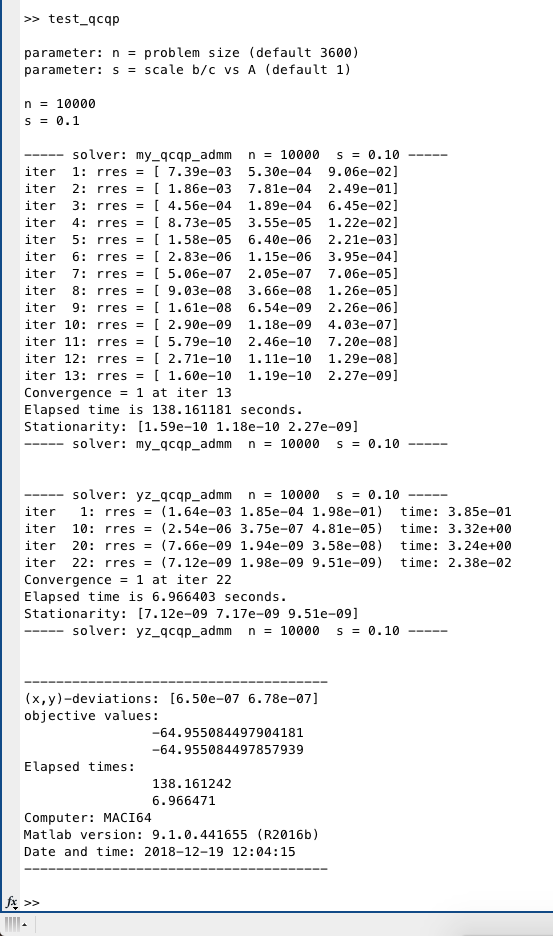
\includegraphics[width=10cm]{F_4/F_1_1.png}
\caption{Historty Inner iteration Numbers for instructor's code}
\end{figure}




\clearpage
\section{Output Figures and Screen Printout for $s=1,n=10000$.}
\subsection{Output Figures ($s=1,n=10000$).}
\begin{figure}[H]
\centering
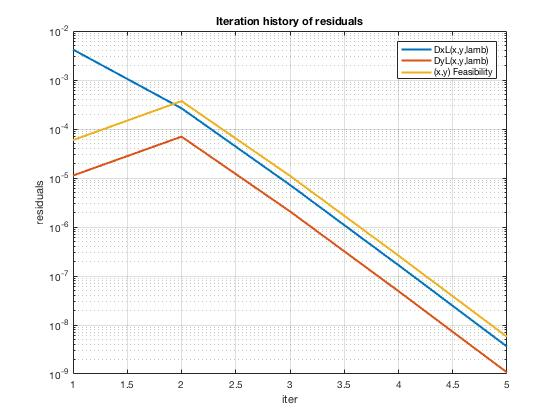
\includegraphics[width=12cm]{F_5/F_1_2.jpg}
\caption{Iteration history residuals for my code}
\end{figure}
\begin{figure}[H]
\centering
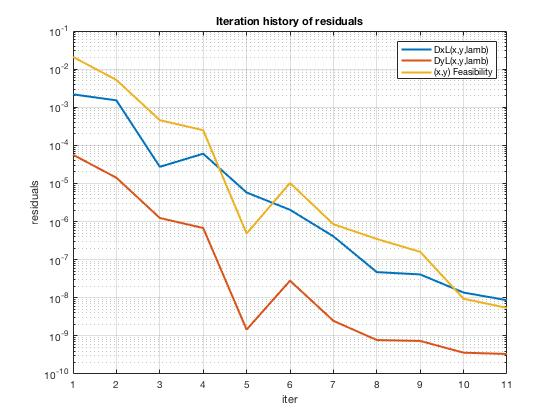
\includegraphics[width=12cm]{F_5/F_1_3.jpg}
\caption{Iteration history residuals for instructor's code}
\end{figure}

\begin{figure}[H]
\centering
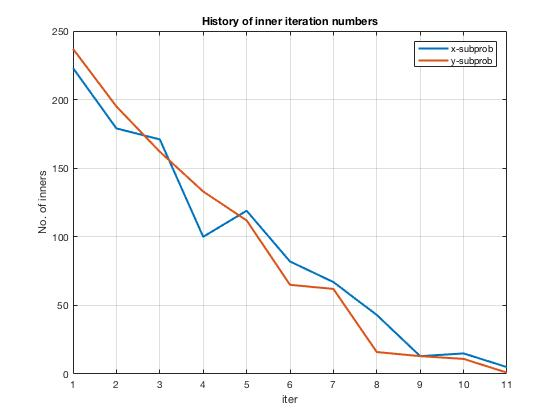
\includegraphics[width=12cm]{F_5/F_1_4.jpg}
\caption{Historty Inner iteration Numbers for instructor's code}
\end{figure}
\subsection{Screen Printout ($s=1,n=10000$).}
\begin{figure}[H]
\centering
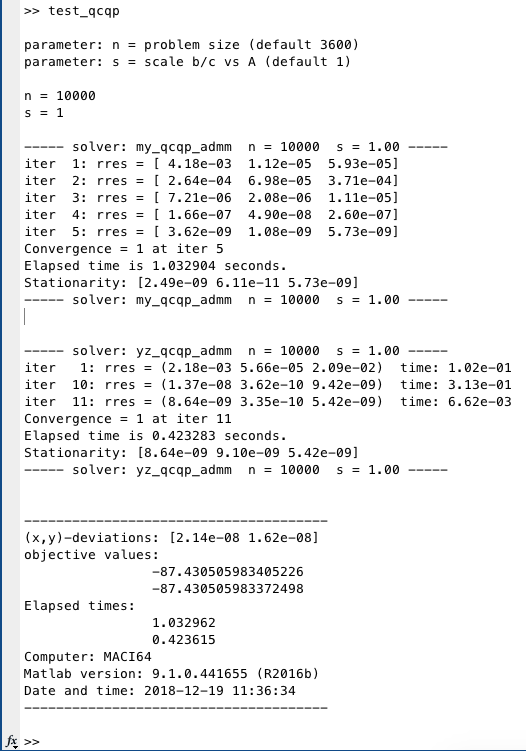
\includegraphics[width=10cm]{F_5/F_1_1.png}
\caption{Historty Inner iteration Numbers for instructor's code}
\end{figure}


\clearpage
\section{Output Figures and Screen Printout for $s=10,n=10000$.}
\subsection{Output Figures ($s=10,n=10000$).}
\begin{figure}[H]
\centering
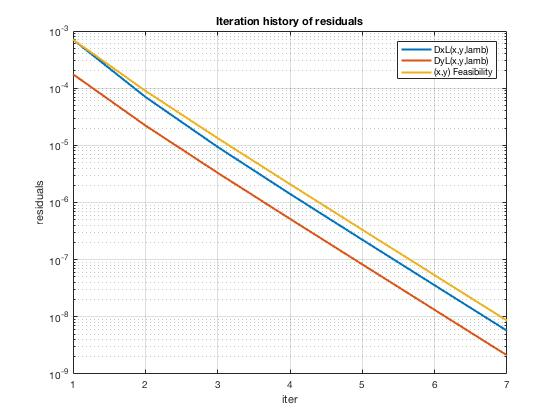
\includegraphics[width=12cm]{F_6/F_1_2.jpg}
\caption{Iteration history residuals for my code}
\end{figure}
\begin{figure}[H]
\centering
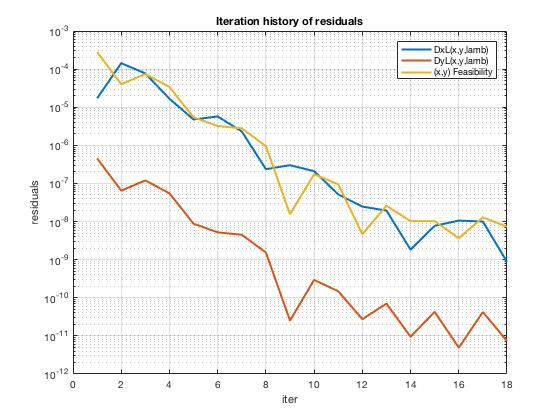
\includegraphics[width=12cm]{F_6/F_1_3.jpg}
\caption{Iteration history residuals for instructor's code}
\end{figure}

\begin{figure}[H]
\centering
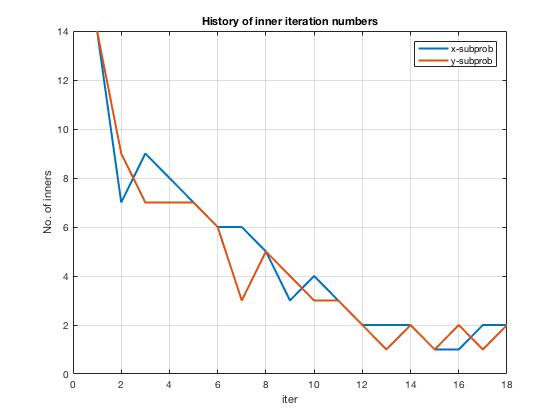
\includegraphics[width=12cm]{F_6/F_1_4.jpg}
\caption{Historty Inner iteration Numbers for instructor's code}
\end{figure}
\subsection{Screen Printout ($s=10,n=10000$).}
\begin{figure}[H]
\centering
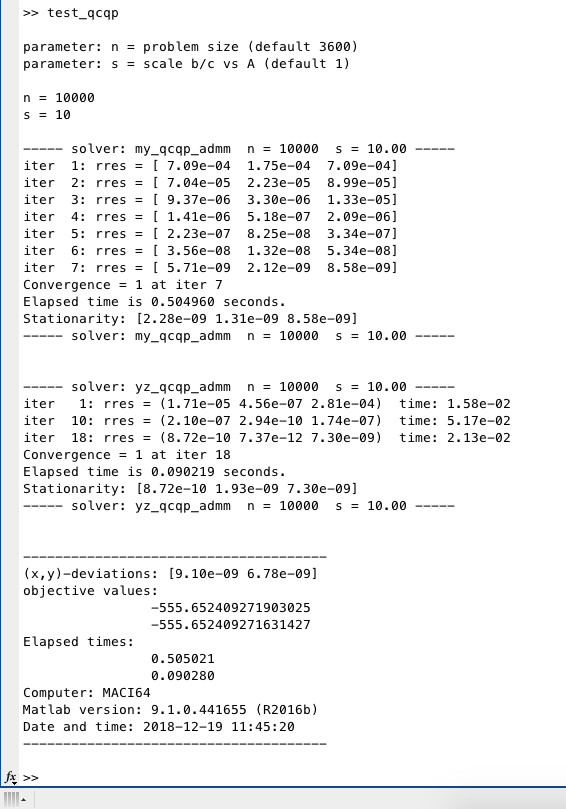
\includegraphics[width=10cm]{F_6/F_1_1.png}
\caption{Historty Inner iteration Numbers for instructor's code}
\end{figure}


\clearpage
\section{Output Figures and Screen Printout for $s=1,n=40000$.}
\subsection{Output Figures ($s=1,n=40000$).}
\begin{figure}[H]
\centering
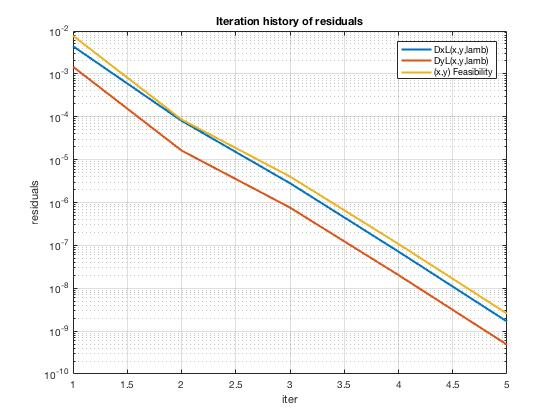
\includegraphics[width=12cm]{F_7/F_1_2.jpg}
\caption{Iteration history residuals for my code}
\end{figure}
\begin{figure}[H]
\centering
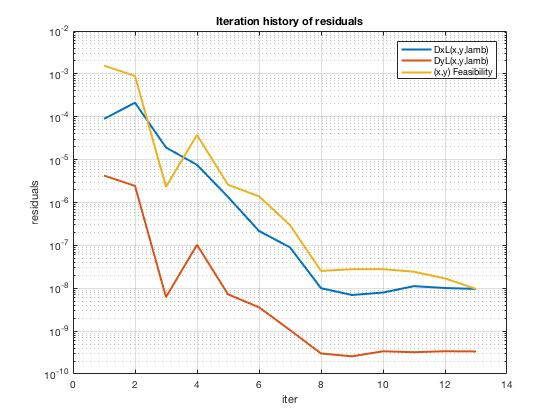
\includegraphics[width=12cm]{F_7/F_1_3.jpg}
\caption{Iteration history residuals for instructor's code}
\end{figure}

\begin{figure}[H]
\centering
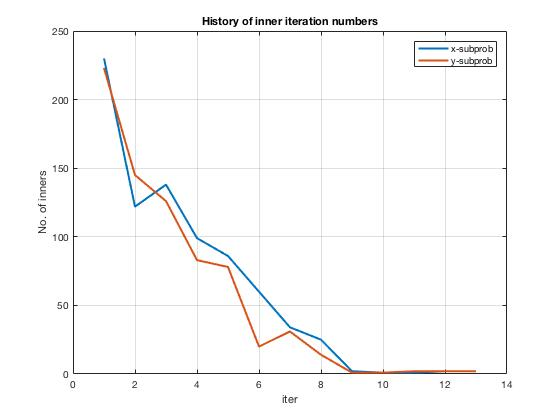
\includegraphics[width=12cm]{F_7/F_1_4.jpg}
\caption{Historty Inner iteration Numbers for instructor's code}
\end{figure}
\subsection{Screen Printout ($s=1,n=40000$).}
\begin{figure}[H]
\centering
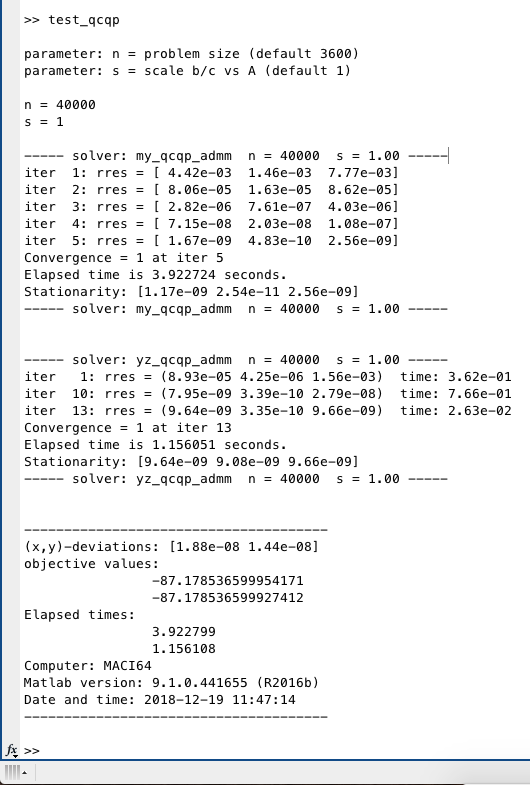
\includegraphics[width=10cm]{F_7/F_1_1.png}
\caption{Historty Inner iteration Numbers for instructor's code}
\end{figure}




\clearpage
\section{Output Figures and Screen Printout for $s=10,n=40000$.}
\subsection{Output Figures ($s=10,n=40000$).}
\begin{figure}[H]
\centering
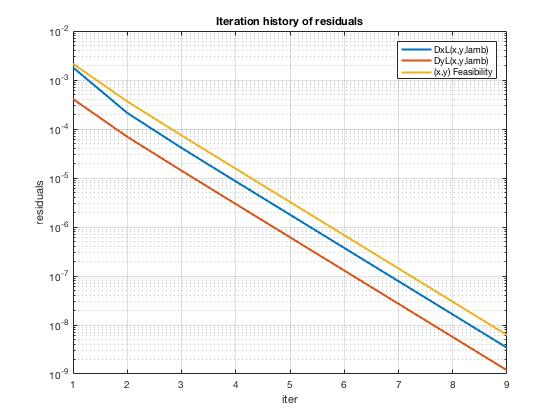
\includegraphics[width=12cm]{F_8/F_1_2.jpg}
\caption{Iteration history residuals for my code}
\end{figure}
\begin{figure}[H]
\centering
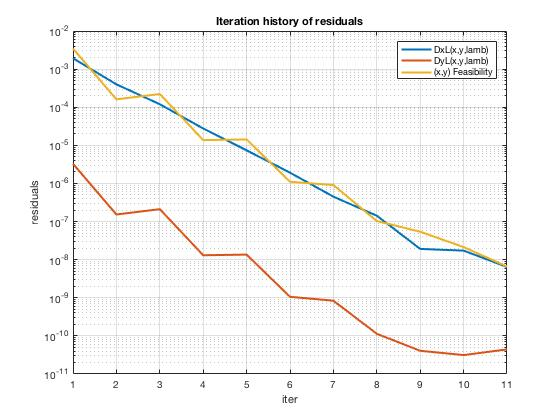
\includegraphics[width=12cm]{F_8/F_1_3.jpg}
\caption{Iteration history residuals for instructor's code}
\end{figure}

\begin{figure}[H]
\centering
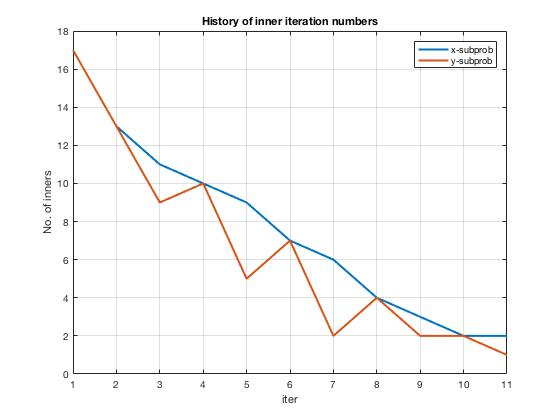
\includegraphics[width=12cm]{F_8/F_1_4.jpg}
\caption{Historty Inner iteration Numbers for instructor's code}
\end{figure}
\subsection{Screen Printout ($s=10,n=40000$).}
\begin{figure}[H]
\centering
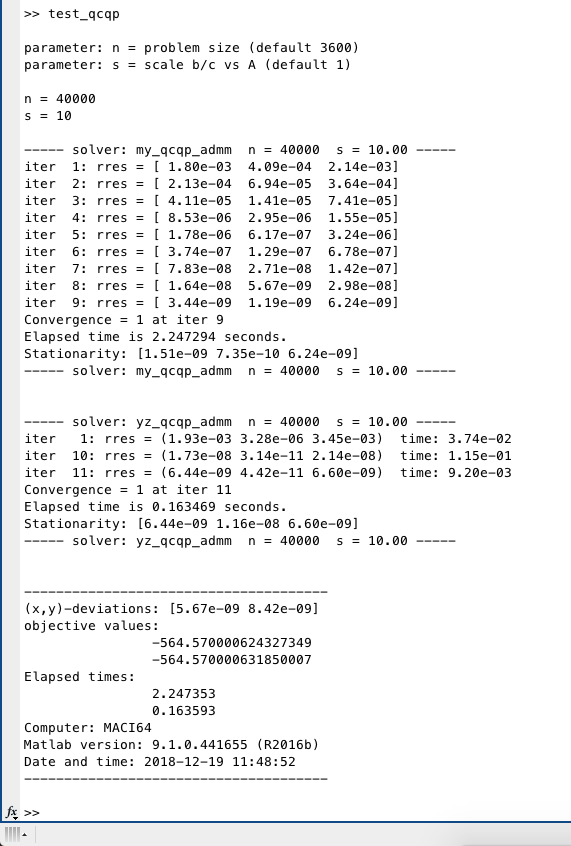
\includegraphics[width=10cm]{F_8/F_1_1.png}
\caption{Historty Inner iteration Numbers for instructor's code}
\end{figure}


\clearpage
\section{Output Figures and Screen Printout for $s=1,n=90000$.}
\subsection{Output Figures ($s=1,n=90000$).}
\begin{figure}[H]
\centering
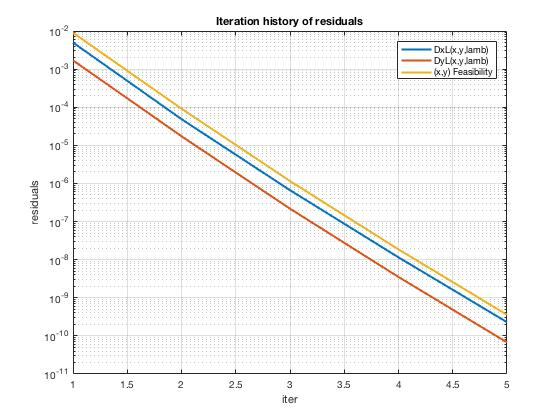
\includegraphics[width=12cm]{F_9/F_1_2.jpg}
\caption{Iteration history residuals for my code}
\end{figure}
\begin{figure}[H]
\centering
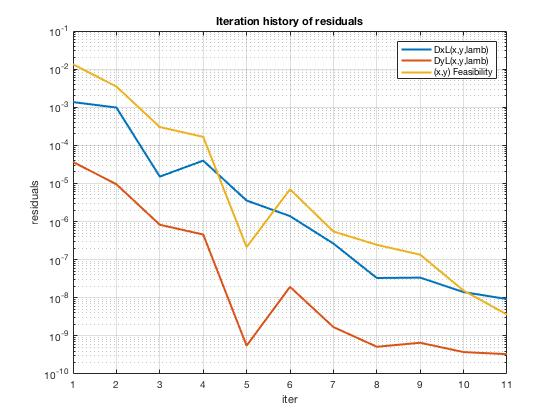
\includegraphics[width=12cm]{F_9/F_1_3.jpg}
\caption{Iteration history residuals for instructor's code}
\end{figure}

\begin{figure}[H]
\centering
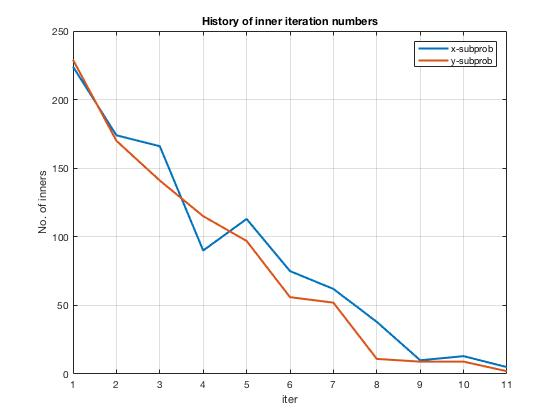
\includegraphics[width=12cm]{F_9/F_1_4.jpg}
\caption{Historty Inner iteration Numbers for instructor's code}
\end{figure}
\subsection{Screen Printout ($s=1,n=90000$).}
\begin{figure}[H]
\centering
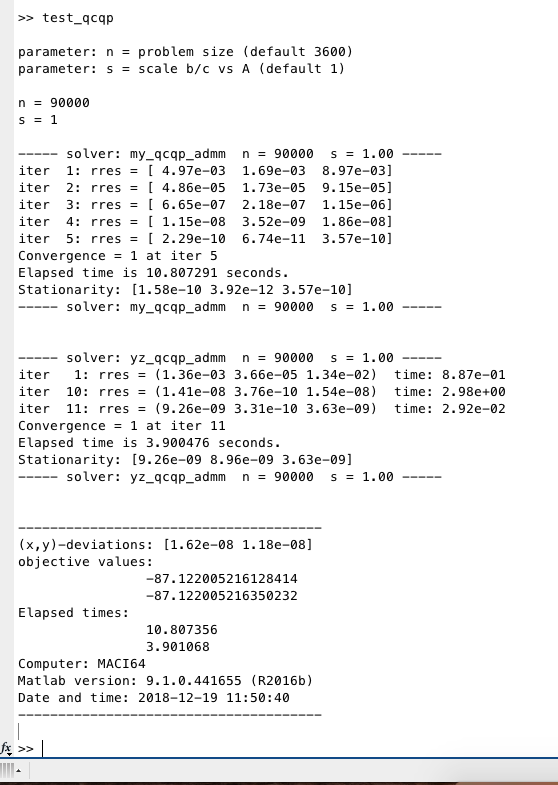
\includegraphics[width=10cm]{F_9/F_1_1.png}
\caption{Historty Inner iteration Numbers for instructor's code}
\end{figure}


\clearpage
\section{Output Figures and Screen Printout for $s=10,n=90000$.}
\subsection{Output Figures ($s=10,n=90000$).}
\begin{figure}[H]
\centering
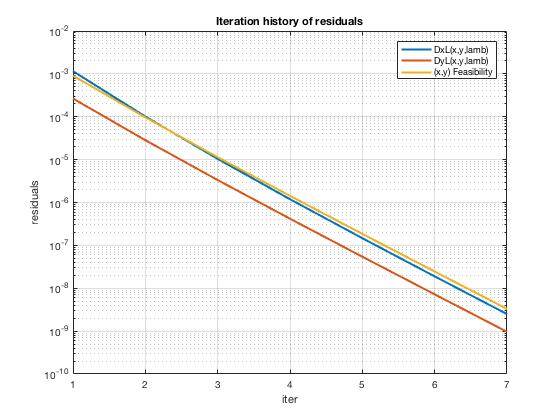
\includegraphics[width=12cm]{F_10/F_1_2.jpg}
\caption{Iteration history residuals for my code}
\end{figure}
\begin{figure}[H]
\centering
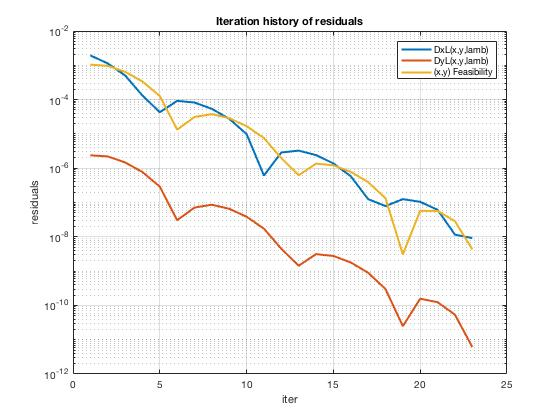
\includegraphics[width=12cm]{F_10/F_1_3.jpg}
\caption{Iteration history residuals for instructor's code}
\end{figure}

\begin{figure}[H]
\centering
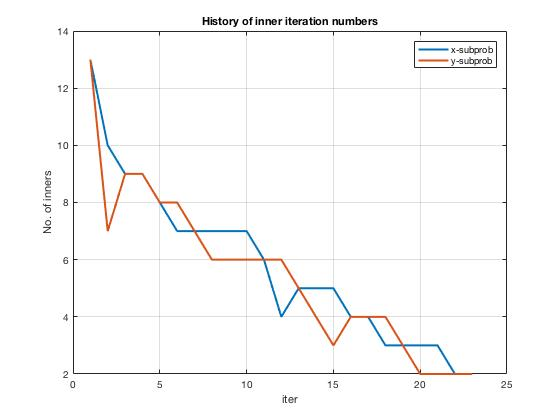
\includegraphics[width=12cm]{F_10/F_1_4.jpg}
\caption{Historty Inner iteration Numbers for instructor's code}
\end{figure}
\subsection{Screen Printout ($s=10,n=90000$).}
\begin{figure}[H]
\centering
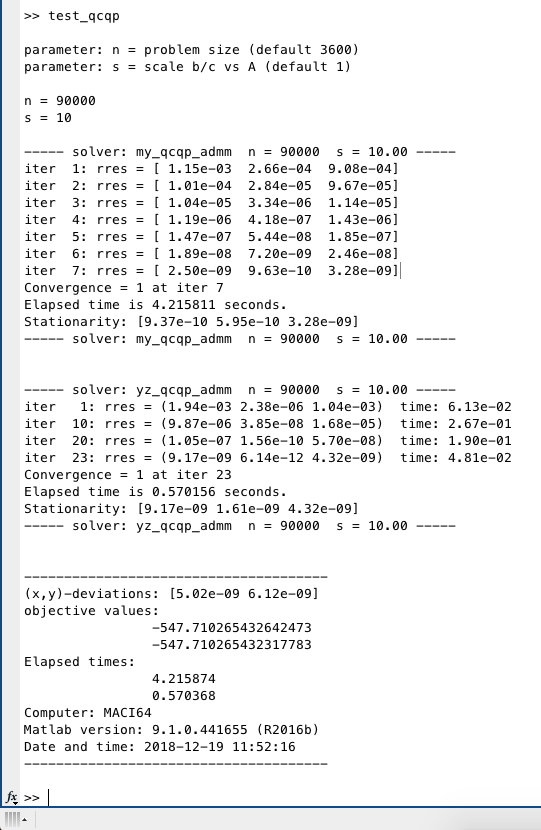
\includegraphics[width=10cm]{F_10/F_1_1.png}
\caption{Historty Inner iteration Numbers for instructor's code}
\end{figure}


\clearpage
\section{Output Figures and Screen Printout for $s=1,n=250000$.}
\subsection{Output Figures ($s=1,n=250000$).}
\begin{figure}[H]
\centering
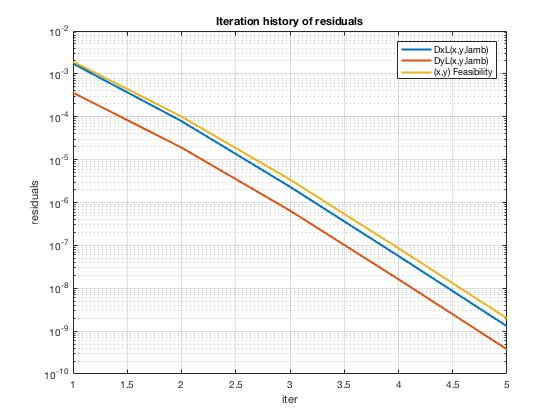
\includegraphics[width=12cm]{F_11/F_1_2.jpg}
\caption{Iteration history residuals for my code}
\end{figure}
\begin{figure}[H]
\centering
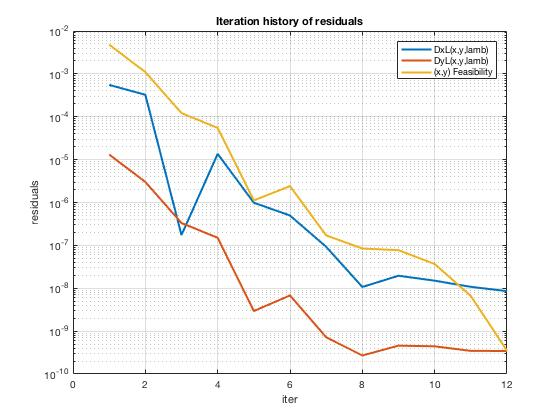
\includegraphics[width=12cm]{F_11/F_1_3.jpg}
\caption{Iteration history residuals for instructor's code}
\end{figure}

\begin{figure}[H]
\centering
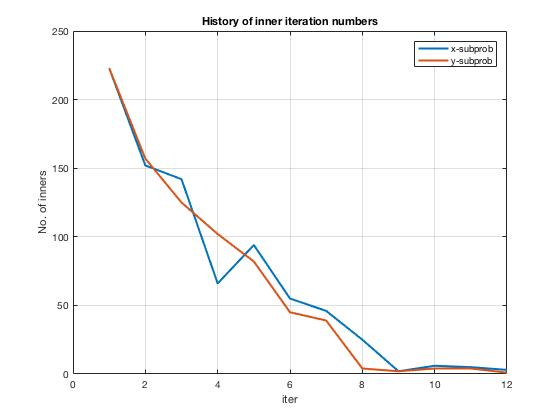
\includegraphics[width=12cm]{F_11/F_1_4.jpg}
\caption{Historty Inner iteration Numbers for instructor's code}
\end{figure}
\subsection{Screen Printout ($s=1,n=250000$).}
\begin{figure}[H]
\centering
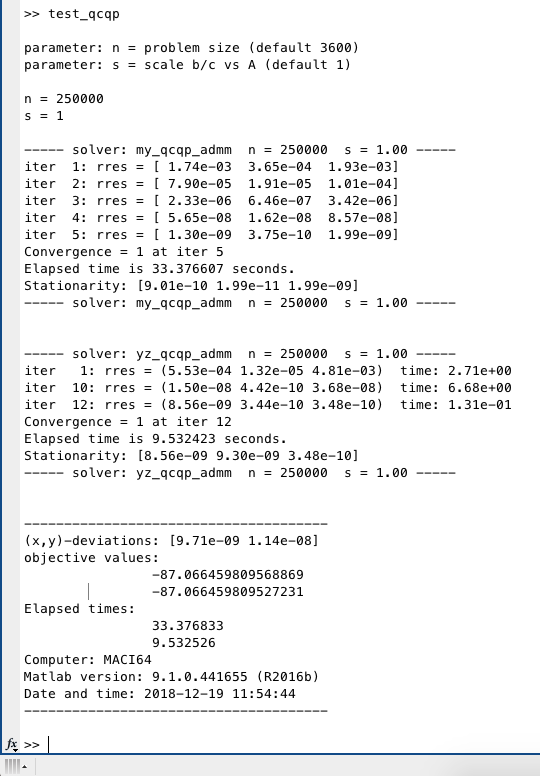
\includegraphics[width=10cm]{F_11/F_1_1.png}
\caption{Historty Inner iteration Numbers for instructor's code}
\end{figure}


\clearpage
\section{Output Figures and Screen Printout for $s=10,n=250000$.}
\subsection{Output Figures ($s=10,n=250000$).}
\begin{figure}[H]
\centering
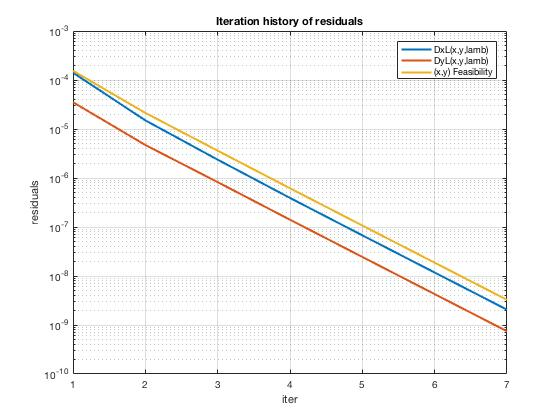
\includegraphics[width=12cm]{F_12/F_1_2.jpg}
\caption{Iteration history residuals for my code}
\end{figure}
\begin{figure}[H]
\centering
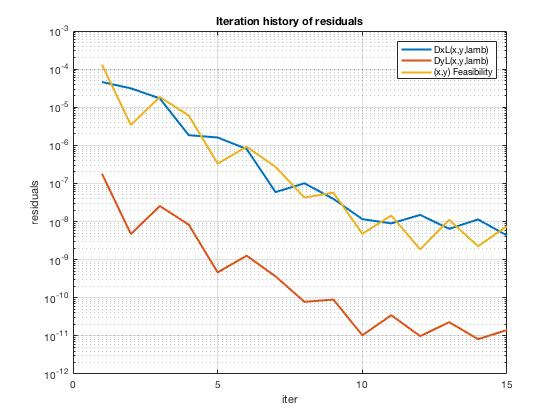
\includegraphics[width=12cm]{F_12/F_1_3.jpg}
\caption{Iteration history residuals for instructor's code}
\end{figure}

\begin{figure}[H]
\centering
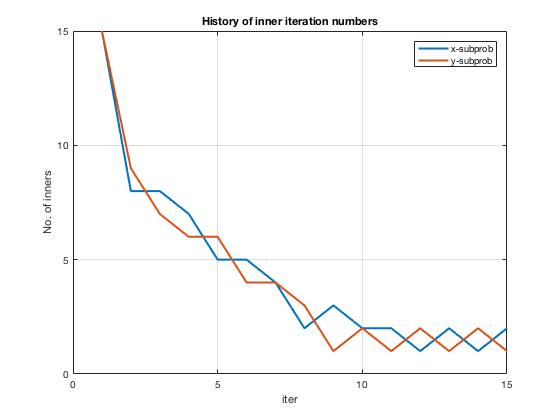
\includegraphics[width=12cm]{F_12/F_1_4.jpg}
\caption{Historty Inner iteration Numbers for instructor's code}
\end{figure}
\subsection{Screen Printout ($s=10,n=250000$).}
\begin{figure}[H]
\centering
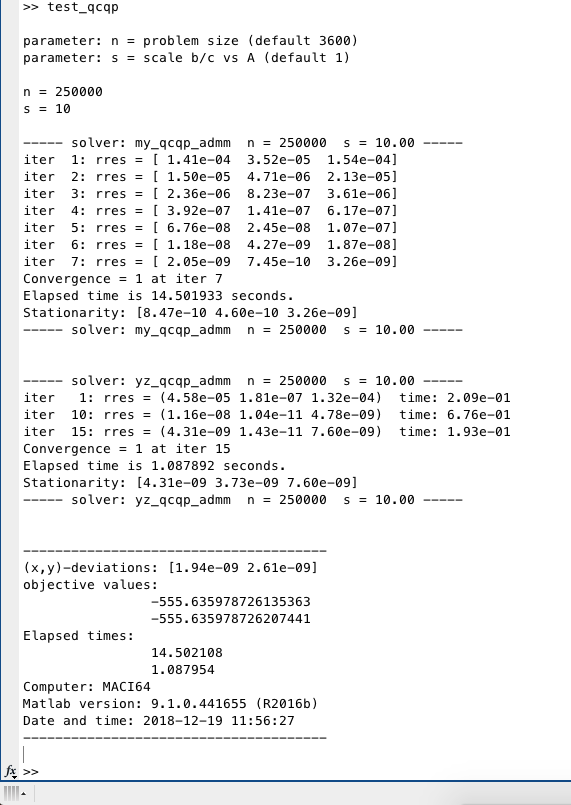
\includegraphics[width=10cm]{F_12/F_1_1.png}
\caption{Historty Inner iteration Numbers for instructor's code}
\end{figure}


\clearpage
\section{Output Figures and Screen Printout for $s=10,n=1000000$.}
\subsection{Output Figures ($s=10,n=1000000$).}
\begin{figure}[H]
\centering
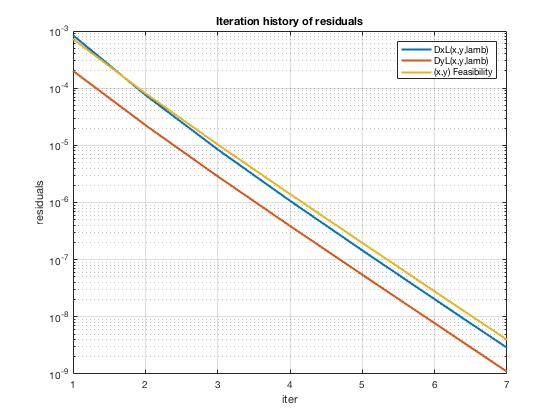
\includegraphics[width=12cm]{F_13/F_1_2.jpg}
\caption{Iteration history residuals for my code}
\end{figure}
\begin{figure}[H]
\centering
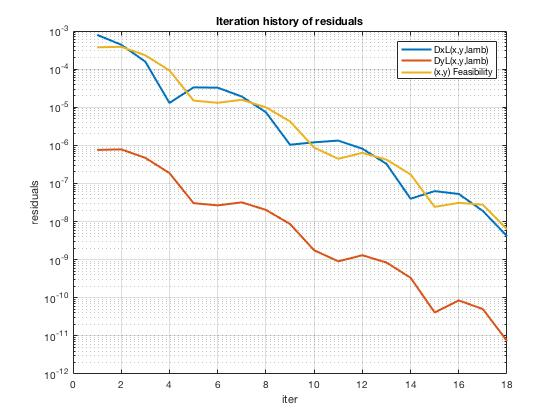
\includegraphics[width=12cm]{F_13/F_1_3.jpg}
\caption{Iteration history residuals for instructor's code}
\end{figure}

\begin{figure}[H]
\centering
\includegraphics[width=12cm]{F_13/F_1_4.jpg}
\caption{Historty Inner iteration Numbers for instructor's code}
\end{figure}
\subsection{Screen Printout ($s=10,n=1000000$).}
\begin{figure}[H]
\centering
\includegraphics[width=10cm]{F_13/F_1_1.png}
\caption{Historty Inner iteration Numbers for instructor's code}
\end{figure}







\end{document}